\documentclass[10pt]{article}
\setlength{\columnsep}{0.75cm}
\usepackage{geometry}
 \geometry{
 letterpaper,
 total={210mm,297mm},
 left=20mm,
 right=20mm,
 top=20mm,
 bottom=20mm,
 }

\usepackage{graphicx}
\usepackage{graphics}
\usepackage{mathrsfs}
\usepackage{dsfont}
\usepackage{caption}
\usepackage{subcaption}
\usepackage{bm} 
% \usepackage[numbers]{natbib}
\usepackage[toc,page]{appendix}
\usepackage{color}
\usepackage{fancyhdr}
\usepackage[english]{babel}
\usepackage{gensymb}
\usepackage[utf8]{inputenc}  
\usepackage[T1]{fontenc}
\usepackage{fancyvrb}
\usepackage{xcolor}
\usepackage{verbatim}
\usepackage{cite}
\usepackage{color}
\usepackage{amsmath}

% \definecolor{Zgris}{rgb}{0.87,0.85,0.85}

% \newsavebox{\BBbox}
% \newenvironment{DDbox}[1]{
% \begin{lrbox}{\BBbox}\begin{minipage}{\linewidth}}
% {\end{minipage}\end{lrbox}\noindent\colorbox{Zgris}{\usebox{\BBbox}} \\\include{BarratHW8.tex}
% [.5cm]}

\newcommand{\ddroit}{\textrm{d}}
% \newcommand{\eexp}{\text{e}}
\newcommand{\ie}{\emph{i.e.}$\;$}
\newcommand{\eg}{\emph{e.g.}$\;$}
\newcommand{\Ptot}{P(A_1\ldots A_L)}

\newcommand{\HRule}{\rule{\linewidth}{0.5mm}}




\begin{document}
	
	\section{Simple model for phylogeny} % (fold)
	\label{sec:simple_model}
	
	Assume a very simple system, with one single spin $\sigma\in\{-1,+1\}$, and hamiltonian $\mathcal{H}^0=h\sigma$. The equilibrium distribution is obviously $P^{eq} = e^{h\sigma}/Z^0$ with $Z^0 = 2\cosh(h)$. $\mathcal{H}^0$ is the model we would like to infer. With a sample of $i.i.d.$ configurations from $P^{eq}$, this is a trivial problem. \\
	Now, consider the case where the available sample comes from the process sketched in Fig. \ref{fig:phylo_sketch}. A number of initial configurations $\sigma^\alpha$, $a\in\{1\ldots K\}$, are chosen -- either at random or from $P^{eq}$. For each initial configuration, a number $N(a)$ of samples are drawn in the following manner: with probability $\mu$, $\sigma$ is drawn from $P^{eq}$, and with probability $(1-\mu)$ it stays equal to $\sigma^a$. In other words, the distribution of $\sigma$ inside one "cluster" $a$ is 
	\begin{equation}
		\label{eq:one_cluster}
		P(\sigma\vert a) = (1-\mu)\delta_{\sigma,\sigma^a} + \mu P^{eq}(\sigma)
	\end{equation}
	The available sample is the union of all configurations of all clusters, resulting in the following distribution 
	\begin{equation}
		\label{eq:all_clusters}
		P^{phylo}(\sigma) = \sum_{a=1}^K p(a)P(\sigma\vert a)
	\end{equation}
	where $p(a)$ is the fraction of configurations in cluster $a$. In the following, it is assumed that the repartition of configurations in clusters is known. In other words, one knows the cluster-wise distributions $P(\sigma\vert a)$.

	\begin{figure}[h!]
	\centering
		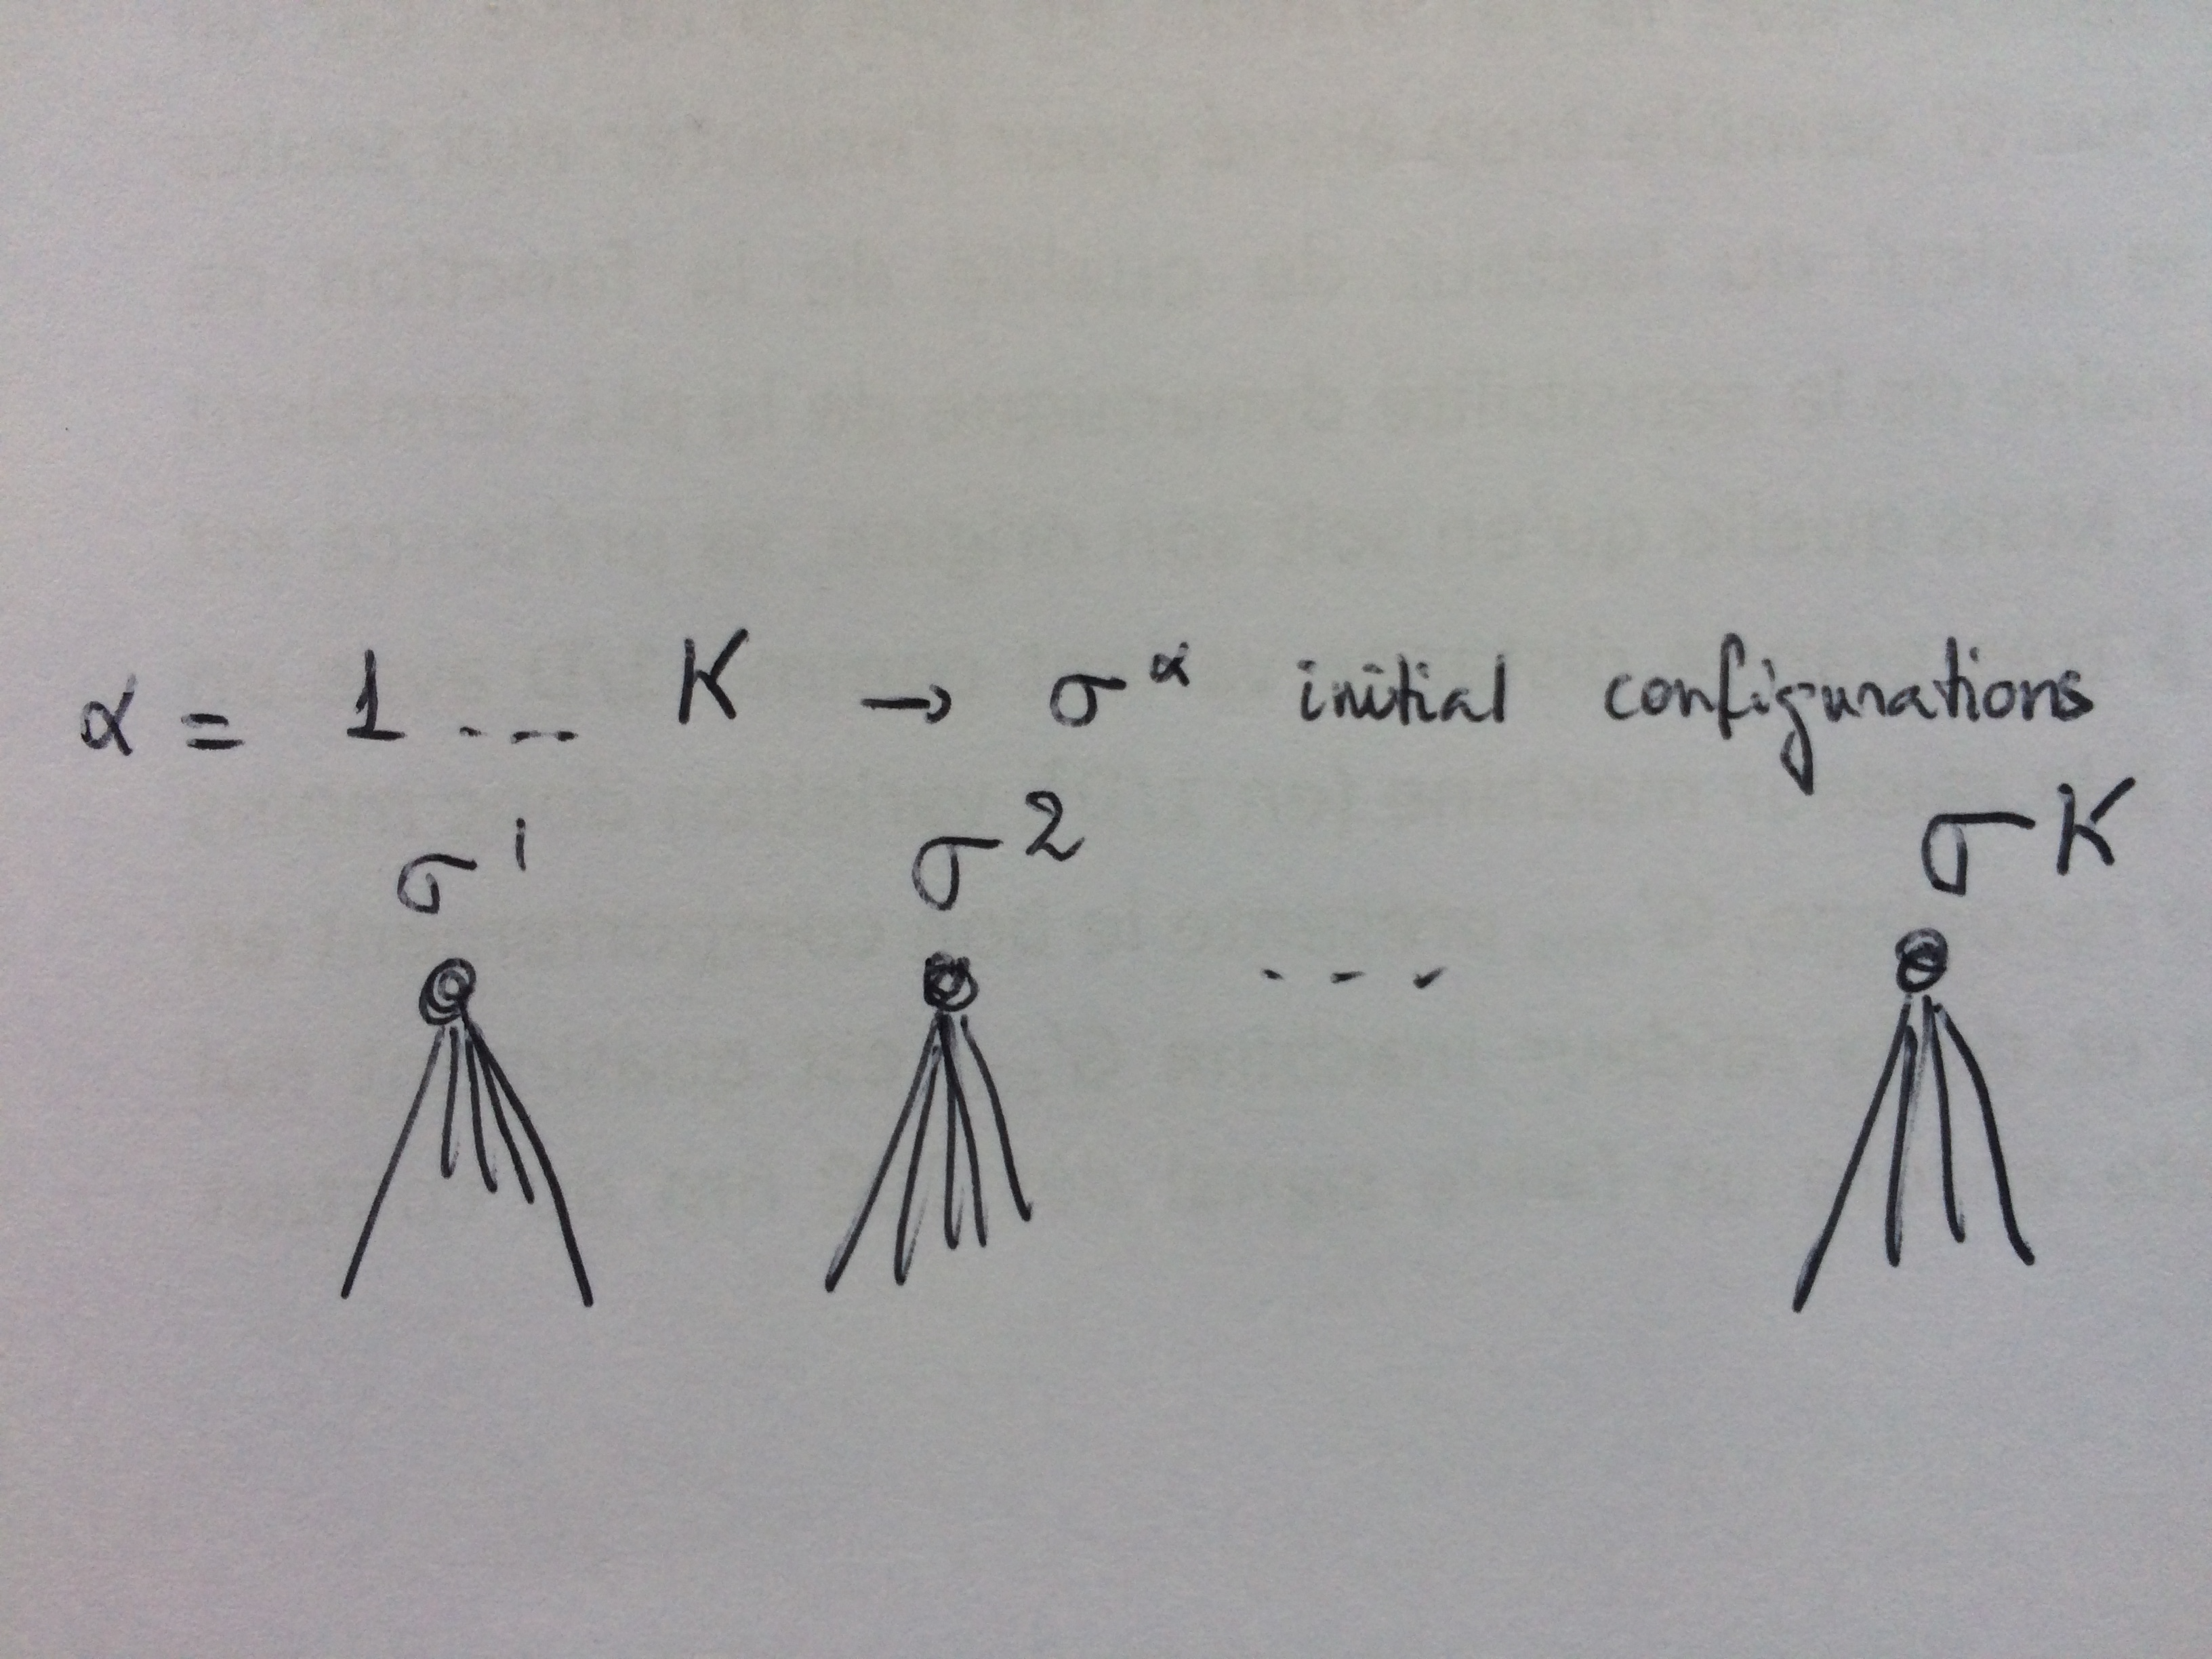
\includegraphics[width = 0.6\textwidth]{./phylo_sketch.png}
		\caption{}
		\label{fig:phylo_sketch}
	\end{figure}  

	% section simple_model (end)

	\section{Naive hidden variable model} % (fold)
	\label{sec:naive_hidden_variable_model}

	Clearly, if one wants to recover the underlying hamiltonian $\mathcal{H}^0$, the biais due to phylogeny needs to be accounted for. The idea of the hidden variable of is to model $P^{phylo}$ with a hamiltonian including a supplementary variable which corresponds to the different phylogenetic clusters. Something like $\tilde{\mathcal{H}} = \mathcal{H}^0(\sigma) + \mathcal{H}^{HN}(\sigma,\alpha)$ -- in the case of a general $N$ spins Ising model, $\mathcal{H}^{HN}$ would not include any interactions between spins, but only with the hidden variable $\alpha$. In practice, one tries to fit $P^{phylo}$ with a distribution of the form 
	\begin{equation}
		\label{eq:HN_basic}
		\tilde{P}(\sigma,\alpha) \propto \exp\left(\xi\sigma + J(\alpha)\sigma + \kappa(\alpha)\right).
	\end{equation}
	Of course, the repartition of sequences in the different clusters $a$ needs to be known in advance.\\
	However, this fitting procedure will not lead to $\xi = h$ in general. It is sufficient to examine the basic case of $K=2$ cluster with initial configurations $\sigma^1$ and $\sigma^{-1}$, where one tries to find parameters $J$ and $\kappa$ so that 
	$$ \frac{\exp\left(\xi\sigma + J\sigma\alpha + \kappa\alpha\right)}{Z(\xi,J,\kappa)} = P^{phylo}(\sigma\vert a=1), $$
	where hidden variable takes values in $\{-1,+1\}$.
	The value of $\xi$ for this fitting procedure can be derived analytically : 
	\begin{equation}
	\label{eq:xi_vs_h}	 	
	\xi = \frac{1}{4}\log\frac{\left( (1-\mu)\delta_{1,\sigma^1} + \mu e^h/Z^0\right)\left( (1-\mu)\delta_{1,\sigma^{-1}} + \mu e^h/Z^0 \right)}{\left( (1-\mu)\delta_{-1,\sigma^1} + \mu e^{-h}/Z^0\right)\left( (1-\mu)\delta_{-1,\sigma^{-1}} + \mu e^{-h}/Z^0 \right)} \neq h
	 \end{equation} 
	This means that the result of this specific parametrization of the hidden variable will not yield the hamiltonian that corresponds to $P^{eq}$.\\
	Number of parameters (corresponding to the hidden node, \ie supplementary parameters with respect to the normal DCA inference) for this method, in the case of $q$ states spins : 
	\begin{itemize}
		\item $J(\alpha,\sigma)$: $(K-1)*(q-1)$ (because of gauge invariance) -- $\times N$ for a full Ising model,
		\item $\kappa(\alpha$): $(K-1)$.
	\end{itemize}

	
	% section naive_hidden_variable_model (end)

	\section{Other parametrization for a hidden variable} % (fold)
	\label{sec:other_parametrization_for_a_hidden_variable}

	One can design a parametrization that better corresponds to equation \ref{eq:all_clusters}:
	\begin{equation}
		\label{eq:HN_better}
		\tilde{P}(\sigma,\alpha) = \sum_{a=1}^K p(\alpha)\left( \mu_\alpha \delta_{\sigma,\sigma^\alpha} + (1-\mu_\alpha)\frac{e^{\xi\sigma}}{2\cosh(\xi)}\right)
	\end{equation}
	The parameters corresponding to the hidden variable are $\sigma^\alpha$, which can have $q$ values for a given $\alpha$, and the scalars $\mu_\alpha$. If fitted perfectly to $P^{phylo}$, this parametrization will obviously give $\xi=h$, recovering the $\mathcal{H}^0$ model. The number of parameters corresponding to the hidden variable in this case is (assuming $p(\alpha)$ is known since sequences are divided into clusters): 
	\begin{itemize}
		\item $\sigma^\alpha$: $K*q$ (not sure if there is some gauge invariance for this kind of model) -- $\times N$ for a full Ising model,
		\item $\mu_\alpha$: $K$.
	\end{itemize}
	This is (almost) the same number as in the previous case. However, those parameters now have an interpretation in terms of phylogeny -- \ie ancestral sequences --, and is more adapted to this very crude phylogeny model.
	
	% section other_parametrization_for_a_hidden_variable (end)

	\section{Calculations} % (fold)
	\label{sec:calculations}
	
	In the case $K=2$, the naive hidden variable model is 
	$$\tilde{P}(\sigma,\alpha) = Z^{-1}\exp(\xi\sigma + J\alpha\sigma + \kappa\alpha)$$
	with hidden variable taking values in $\{-1,+1\}$.\\
	If one knows the repartition of configurations in cluster, then the distribution of data is 
	$$P^{phylo}(\sigma,a) = p(a)\left((1-\mu)\delta_{\sigma,\sigma^a} + \mu\frac{e^{h\sigma}}{Z^0}\right).$$
	One tries to find values $\{\xi,J,\kappa\}$ such that $\tilde{P}(\sigma,\alpha) = P^{phylo}(\sigma,\alpha)$. Writing this equality for all combinations of $\sigma$ and $\alpha$, one gets 
	\begin{align}
		Z^{-1}e^{\xi + J + \kappa} &= P^{phylo}(1,1)\\
		Z^{-1}e^{\xi - J - \kappa} &= P^{phylo}(1,-1)\\
		Z^{-1}e^{-\xi - J + \kappa} &= P^{phylo}(-1,1)\\
		Z^{-1}e^{-\xi + J - \kappa} &= P^{phylo}(-1,-1).\\
	\end{align}
	This immediately gives
	$$\xi = \frac{1}{4}\log\frac{P^{phylo}(1,1)P^{phylo}(1,-1)}{P^{phylo}(-1,1)P^{phylo}(-1,-1)}.$$
	In the particular case where $p(a) = 1/2$, this is the same as equation \ref{eq:xi_vs_h}. 
	% section calculations (end)

\end{document}